% =====================================================================
%  ch2_motivation.tex — §2 动机与与其他方法的比较
% =====================================================================
\section{动机与与其他方法的比较}\label{s:pantsmotivate}

本节讨论平面曲线的 Landau--Ginzburg 镜像的辛几何的若干特征，特别聚焦于 $(\C^3,-xyz)$（裤子的镜像）这一情形。这些材料有助于理解 §\ref{s:Amodel} 所述构造的来由，以及它与其他方法的若干关键差别；但本节并非主要论证的组成部分。想直接读到构造的确切表述与定理~\ref{thm:main} 的证明的读者，可以完全跳过本节。

\subsection{动机：裤子的镜像}\label{ss:pantsmirror}

我们先考察 Landau--Ginzburg 模型 $(\C^3,-xyz)$ 的辛几何，以及它在裤子（例~\ref{ex:pants}）情形下如何反映在我们的 A 模型构造之中。

把 Landau--Ginzburg 模型的辛几何归结为其临界点集的辛几何，这一普遍想法来自两个已被很好理解的模型：Lefschetz 纤维化，以及理解得稍差、但更接近本文情形的 Morse--Bott 纤维化。例如，\cite{AAK} 的构造为一条光滑椭圆曲线 $X$（嵌入环面曲面）配置一个三维 Landau--Ginzburg 模型 $(Y,W)$，其奇点是沿一条光滑椭圆曲线 $M=\crit(W)\subset Y$ 的 Morse--Bott 奇点，而 $M$ 事实上就是 $X$ 的「通常」镜像。于是我们可以把 $M$ 的 Fukaya 范畴的一个对象（即带局部系统的简单闭曲线）升级为 $Y$ 中的一个拉格朗日\textbf{刺形}（thimble）：沿一条从 $W$ 的临界值（原点）通往 $+\infty$ 的弧作平行移动即可得到。确切地说，对 $L\in\F(M)$ 配置 $\mathcal{T}(L)\in\F(Y,W)$，即由 $Y$ 中满足下述条件的点组成的可容许拉格朗日：$\Re(W)$ 关于某个 K\"ahler 度量的负梯度流收敛到 $L$ 上一点（并带上拉回的局部系统）。此例给出函子 $\mathcal{T}:\F(M)\to\F(Y,W)$，它实际上是等价；不过要注意，对一般的 Morse--Bott 纤维化，情形可能略为复杂（例如见 \cite[推论 7.8]{AAK}）。

我们关心的情况落在 Morse--Bott 框架之外：考虑 Landau--Ginzburg 模型 $(\C^3,-xyz)$ 及其纤维化缠绕 Fukaya 范畴。$\F(\C^3,-xyz)$ 的对象是 $\C^3$ 的可容许拉格朗日子流形，其在投影 $W=-xyz:\C^3\to\C$ 下的像在无穷远处由一条或多条指向 $\Re(W)\to+\infty$ 的射线组成；态射则涉及 Hamilton 扰动，这些扰动在 $W$ 的纤维内于无穷远处缠绕拉格朗日，并把纤维化底空间中的射线沿逆时针方向略作推移 \cite{AA}。

Landau--Ginzburg 模型的 Fukaya 范畴与正则纤维的 Fukaya 范畴（此处即 $(\C^*)^2$ 的缠绕 Fukaya 范畴）通过一对球函子相联系 \cite{AG,AS}，通常记作 $\cup$ 与 $\cap$，我们简述如下。在对象上，杯函子（cup functor，也称 Orlov 函子）
\[
\cup:\W((\C^*)^2)\to\F(\C^3,-xyz)
\]
把 $(\C^*)^2\simeq\{xyz=1\}=W^{-1}(-1)$ 中的拉格朗日子流形 $\ell$ 沿 $W=-xyz$ 的纤维、在底空间一条 U 形弧上作平行移动，得到 $\C^3$ 中的可容许拉格朗日子流形 $\cup\ell$。帽函子（cap functor）
\[
\cap:\F(\C^3,-xyz)\to\Tw\,\W((\C^*)^2)
\]
把可容许拉格朗日 $\mathbf{L}\subset\C^3$ 限制为其在 $\Re(W)\to\infty$ 的各端中的纤维化拉格朗日；若只有一个这样的端，就得到 $\W((\C^*)^2)$ 的一个对象；否则得到一个由 $\mathbf{L}$ 各端中对象构成的扭曲复形，其连接微分由 $\C^3$ 中以 $\mathbf{L}$ 为边界的全纯圆盘计数给出（带一个朝向 $\Re(W)\to\infty$ 的出射带状端）。\cite{AA} 的论证以与这些函子相容的方式证明了裤子的同调镜像对称（以及其他很仿射的超曲面），即：

\begin{theo}[\cite{AA}]
$\F(\C^3,-xyz)$ 等价于裤子 $X=\{(x_1,x_2)\in(K^*)^2\,|\,1+x_1+x_2=0\}$ 的导出范畴，且有交换图表
\[
\xymatrix{
\!\!\!\!\Tw\,\F(\C^3,-xyz) \ar@<.5ex>[r]^{\cap} \ar[d]^{\simeq}
& \Tw\,\W((\C^*)^2) \ar@<.5ex>[l]^{\cup}\ar[d]^{\simeq} \\
\Perf(X)\ar@<.5ex>[r]^{i_*} & \Perf((K^*)^2) \ar@<.5ex>[l]^{i^*}
}
\]
即函子 $\cap$ 与 $\cup$ 在镜像对称下对应于 $X$ 与环绕空间 $(K^*)^2$ 的导出范畴之间的包含函子与限制函子 $i_*$ 与 $i^*$。
\end{theo}

临界点集 $M=\crit(W)$ 是 $\C^3$ 中坐标轴之并，因而并不光滑；但 $W$ 的奇点在原点之外都是 Morse--Bott 的。给定 $M$ 光滑部分中一个嵌入拉格朗日子流形 $L_p$，可以沿实正轴作平行移动，构造刺形 $\mathcal{T}(L_p)\subset\C^3$。例如取 $\C^3$ 的标准 K\"ahler 形式，从 $L_p=\{(x,0,0)\,|\,|x|=r\}\subset M$ 出发，得到拉格朗日
\[
\mathcal{T}(L_p)=\bigl\{(x,y,z)\in\C^3\,\big|\,|x|^2-r^2=|y|^2=|z|^2,\ -xyz\in\R_{\ge 0}\bigr\}
\]
（\cite{AA} 出于技术原因使用了另一个环面 K\"ahler 形式，这与我们的讨论无关）。可以给 $\mathcal{T}(L_p)$ 配上 Novikov 域 $K$ 上一个（酉的，即保值）秩 $1$ 局部系统，并且还应给它配一个界定余链（bounding cochain），以消去由 $\mathcal{T}(L_p)$ 所界定的全纯圆盘（即 $x$ 轴中半径为 $r$ 的圆盘，记其辛面积为 $A$，以及它的多重覆叠）带来的 Floer 理论障碍。这样就得到 $\F(\C^3,-xyz)$ 中所谓的 Aganagic--Vafa 拉格朗日膜，它是裤子 $X=\{1+x_1+x_2=0\}$ 上一点 $p$ 的摩天楼层 $\cO_p$ 的镜像，其中 $\val(x_1(p))=A$；坐标 $(x_1,x_2)$ 的值依赖于局部系统与界定余链的选取。

消没圈，即无穷远处的边界 $\Lambda_p=\cap\mathcal{T}(L_p)$，是 $(\C^*)^2$ 中一个带秩 $1$ 局部系统的拉格朗日环面（由于消障的界定余链，其和乐即使在界定 $\mathcal{T}(L_p)$ 内部圆盘的那个 $S^1$ 因子上也非平凡）；它实际上是 $(K^*)^2$ 中点 $p$ 的摩天楼层的镜像，这与「$\cap$ 在镜像对称下对应 $i_*$」的预期相符。

对应于 $X$ 的结构层的对象，应当与每个点对象恰好相交一次；因此自然会考虑奇异拉格朗日
\[
L_0=\bigcup_{i=1}^3\R_{\ge 0},
\]
即 $M$ 三个分量中正实轴之并。用平行移动可以从 $L_0$ 构造出 $(\C^3,-xyz)$ 中一个分段线性的拉格朗日闭链，它与无穷远处光滑纤维 $\{-xyz=c\gg 0\}$ 的交 $\Lambda_0^{PL}$（「PL 消没圈」）是三个半无限圆柱 $\{|x|\ge|y|=|z|,\ \arg(x)=0\}$、$\{|y|\ge|x|=|z|,\ \arg(y)=0\}$、$\{|z|\ge|x|=|y|,\ \arg(z)=0\}$ 与环面 $\{|x|=|y|=|z|\}$ 的两个三角部分之并。然而，如何修改这一构造以得到 $\C^3$ 中的光滑可容许拉格朗日，并不清楚。

因此，\cite{AA} 的论证绕开了构造刺形的尝试，转而考虑对象 $\mathbf{L}_0=\cup\ell_0\in\F(\C^3,-xyz)$：它由 $\ell_0=(\R_+)^2\subset(\C^*)^2$ 沿复平面中一条 U 形弧平行移动得到，见图~\ref{fig:pantsLGmirror}。

\begin{figure}[t]
\centering
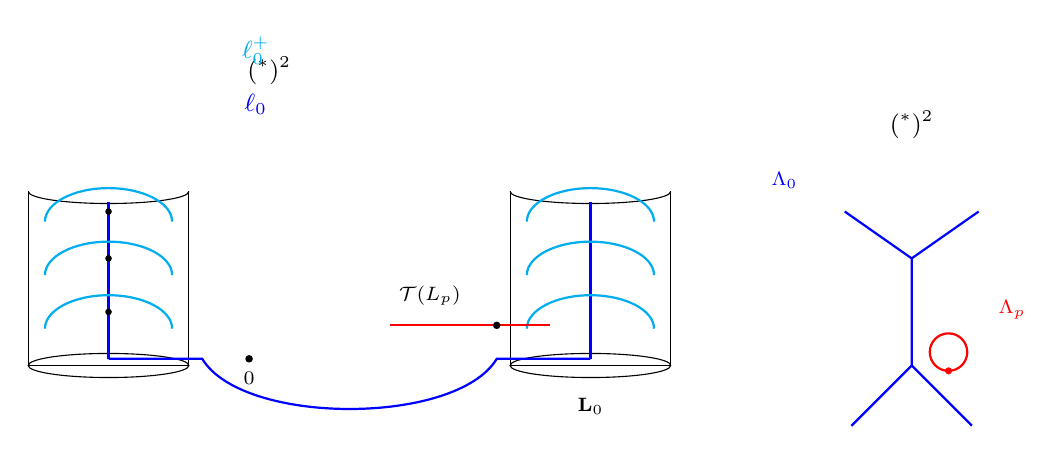
\begin{tikzpicture}[scale=0.85]
% 左：两个纤维，L_0 与 T(L_p)
\draw (-1.2,4.4) node {\small $(\C^*)^2$};
\draw[blue] (-1.4,3.9) node {\small $\ell_0$};
\draw[cyan] (-1.4,4.7) node {\small $\ell_0^+$};
% 左柱
\draw (-3.6,0) ellipse (1.2 and 0.18);
\draw (-3.6,0) -- (-4.8,0); \draw (-3.6,0) -- (-2.4,0);
\draw (-4.8,0) -- (-4.8,2.6); \draw (-2.4,0) -- (-2.4,2.6);
\draw (-4.8,2.6) arc (180:360:1.2 and 0.18);
\draw[blue,thick] (-3.6,0.1) -- (-3.6,2.45);
\foreach \y in {0.8,1.6,2.3} \fill (-3.6,\y) circle (1.4pt);
\draw[cyan,thick] (-4.55,0.55) arc (180:0:0.95 and 0.5);
\draw[cyan,thick] (-4.55,1.35) arc (180:0:0.95 and 0.5);
\draw[cyan,thick] (-4.55,2.15) arc (180:0:0.95 and 0.5);
% 右柱
\draw (3.6,0) ellipse (1.2 and 0.18);
\draw (3.6,0) -- (2.4,0); \draw (3.6,0) -- (4.8,0);
\draw (2.4,0) -- (2.4,2.6); \draw (4.8,0) -- (4.8,2.6);
\draw (2.4,2.6) arc (180:360:1.2 and 0.18);
\draw[blue,thick] (3.6,0.1) -- (3.6,2.45);
\draw[cyan,thick] (2.65,0.55) arc (180:0:0.95 and 0.5);
\draw[cyan,thick] (2.65,1.35) arc (180:0:0.95 and 0.5);
\draw[cyan,thick] (2.65,2.15) arc (180:0:0.95 and 0.5);
% 中间：U 形弧连接
\draw[blue,thick] (-3.6,0.1) -- (-2.2,0.1) .. controls (-1.6,-0.9) and (1.6,-0.9) .. (2.2,0.1) -- (3.6,0.1);
\fill (-1.5,0.1) circle (1.6pt);
\node[below] at (-1.5,0.05) {\scriptsize $0$};
% 红色刺形
\draw[red,thick] (0.6,0.6) -- (3.0,0.6);
\fill (2.2,0.6) circle (1.6pt);
\node[above] at (1.2,0.75) {\scriptsize $\mathcal{T}(L_p)$};
\node[below] at (3.6,-0.35) {\scriptsize $\mathbf L_0$};
% 右图：热带裤子
\begin{scope}[shift={(8.4,0)}]
\draw (0,3.6) node {\small $(\C^*)^2$};
\draw[blue,thick] (0,0) -- (0,1.6) -- (-1.0,2.3);
\draw[blue,thick] (0,1.6) -- (1.0,2.3);
\draw[blue,thick] (0,0) -- (0.9,-0.9);
\draw[blue,thick] (0,0) -- (-0.9,-0.9);
\draw[red,thick] (0.55,0.2) circle (0.28);
\fill[red] (0.55,-0.08) circle (1.5pt);
\node[red,above] at (1.5,0.55) {\scriptsize $\Lambda_p$};
\node[blue,above] at (-1.9,2.5) {\scriptsize $\Lambda_0$};
\end{scope}
\end{tikzpicture}
\caption{左：$\mathbf{L}_0=\cup\ell_0\in\F(\C^3,-xyz)$ 与刺形 $\mathcal{T}(L_p)$，分别位于 $W$ 的两个纤维中，$\mathbf{L}_0$ 沿底空间中的 U 形弧把 $\ell_0$ 平行移动到 $\ell_0^+$。右：热带拉格朗日裤子 $\Lambda_0\simeq\cap\mathbf{L}_0\subset(\C^*)^2$ 与 $\Lambda_p=\cap\mathcal{T}(L_p)$。}\label{fig:pantsLGmirror}
\end{figure}

\cite{AA} 中同调镜像对称的证明依靠直接计算：$\mathbf{L}_0$ 的纤维化缠绕 Floer 复形为
\[
\End(\mathbf{L}_0)\simeq
\left\{CW^*(\ell_0,\ell_0)[1]\xrightarrow{\ \partial\ }CW^*(\ell_0,\ell_0)\right\}\simeq
\left\{K[x_1^{\pm 1},x_2^{\pm 1}][1]\xrightarrow{\ 1+x_1+x_2\ }K[x_1^{\pm 1},x_2^{\pm 1}]\right\},
\]
且其上同调代数与裤子的函数环一致。（复形的两项对应于图~\ref{fig:pantsLGmirror} 左侧 $W$ 的两个纤维中 $\mathbf{L}_0$ 与其正扰动 $\mathbf{L}_0^+$ 的交点；每一项都等于 $\ell_0$ 在 $(\C^*)^2$ 中的缠绕 Floer 上同调，而连接微分是对纤维化底空间中可见的大二边形上的全纯截面计数。）

这一计算虽然证明了裤子 $X$ 与 Landau--Ginzburg 模型 $(\C^3,-xyz)$ 的同调镜像对称，却没有说明 $\mathbf{L}_0$ 的自同态如何与 $M$ 中 $L_0=\bigcup_{i=1}^3\R_{\ge 0}$ 的某个缠绕 Floer 同调版本相联系（比较图~\ref{fig:pantsmirror}）：$HW^0_M(L_0,L_0)$ 带有一组对应于 Floer 生成元的、在标量意义下典范的基，而 $H^0\End(\mathbf{L}_0)$ 是 $HW^0_{(\C^*)^2}(\ell_0,\ell_0)\simeq K[x_1^{\pm 1},x_2^{\pm 1}]$ 商去由 $1+x_1+x_2$ 生成的理想，并没有优先的基。

更有希望的进路来自如下观察：尽管 $\mathbf{L}_0$ 在 $\Re(W)\to+\infty$ 处有两个端，从而在帽函子下映为扭曲复形而非单个拉格朗日，具体地说是映射锥
\[
\bigl\{\ell_0[1]\xrightarrow{\ 1+x_1+x_2\ }\ell_0\bigr\}\in\Tw\,\W((\C^*)^2),
\]
但该扭曲复形实际上可以用 $(\C^*)^2$ 中一个嵌入拉格朗日 $\Lambda_0$ 几何地表示：这就是 Hicks、Matessi 与 Mikhalkin 各自独立引入的\textbf{热带拉格朗日裤子} \cite{Hicks,Matessi,Mikhalkin}。并非巧合，$\Lambda_0$ 事实上是 PL 消没圈 $\Lambda_0^{PL}$ 的光滑化。要注意，Hicks 的构造把热带拉格朗日裤子明确实现为 $\ell_0$ 与其在纤维化 $W$ 的单值性下的像之间的映射锥，这就使 $\cap\mathbf{L}_0\simeq\Lambda_0$ 变得显然 \cite{Hicks}。这一点之所以相关，是因为帽函子诱导的映射 $\Hom(\mathbf{L}_0,\mathbf{L}_0)\to\Hom(\cap\mathbf{L}_0,\cap\mathbf{L}_0)$ 是单射（事实上这对 $\F(\C^3,-xyz)$ 的每个对象都成立，因为涉及伴随 $\cup\cap\to\id$ 余单位的函子正合三角是可裂的）。因此 $H^*\End(\mathbf{L}_0)$ 自然地成为 $(\C^*)^2$ 中缠绕 Floer 上同调 $HW^*(\Lambda_0,\Lambda_0)$ 的直和项，具体地说是零次部分 $HW^0(\Lambda_0,\Lambda_0)$。在镜像对称下，这对应于 $\Hom^0(i_*\cO_X,i_*\cO_X)\simeq\End(\cO_X)$。总结如下：

\begin{prop}\label{prop:HW0}
热带拉格朗日裤子 $\Lambda_0\subset(\C^*)^2$ 的零次缠绕 Floer 上同调 $HW^0(\Lambda_0,\Lambda_0)$ 作为环同构于 $\End(\cO_X)$，即裤子 $X$ 的函数环。
\end{prop}
% [Tutor Note: 直觉] 这里 $\Lambda_0$ 与上一段的 thimble $\cT(L_p)$ 是同一对象的两种极限：$\cT(L_p)$ 是 $(\C^3,-xyz)$ 中的精确拉格朗日，$\Lambda_0$ 则是它在 $|x_1|,|x_2|\to\infty$ 的 SYZ 极限下退化成的热带骨架。取零次部分 $HW^0$ 相当于只看 thimble 上「沿纤维方向常值」的那部分态射，因而 $HW^0(\Lambda_0,\Lambda_0)$ 只是 $H^*\End(\cT(L_p))$ 的直和项，而非全部。依据：原文 §2.1 与 \cite{Hicks,Matessi,Mikhalkin}，并见本工程 01_通读笔记。

于是，我们对 $M$ 中 $L_0$ 的缠绕 Floer 上同调的定义，是由与 $(\C^*)^2$ 中 $\Lambda_0$ 的零次缠绕 Floer 上同调的类比所驱动的。$HW^0(\Lambda_0,\Lambda_0)$ 有一个生成元 $e$，对应缠绕 Hamilton 函数的极小值，代表 Floer 乘积的单位元；在 $\Lambda_0$ 的三条腿中，每条腿还有一列无穷多个生成元 $\theta_{i,k}$，$k\ge 1$，$1\le i\le 3$（对应于在 $\arg(x)$（相应地 $\arg(y)$、$\arg(z)$）方向上缠绕 $k$ 圈的 Hamilton 流轨道）。

\begin{lemma}\label{l:floergens_as_rationalfunctions}
在同构 $HW^0(\Lambda_0,\Lambda_0)\simeq\End(\cO_X)$ 下，Floer 生成元 $\theta_{i,k}$ 对应于 $X$ 上一个正则函数，它作为 $\PP^1$ 上的有理函数，在第 $i$ 个穿孔点有 $k$ 阶极点，且无其他极点。
\end{lemma}

\begin{proof}
回忆 $\Lambda_0$ 的缠绕 Floer 复形是 Floer 复形 $CF^*(\Lambda_n,\Lambda_0)$ 的正向极限，其中 $\Lambda_n$ 是 $\Lambda_0$ 在某个 Hamilton 微分同胚下的像，该微分同胚把三条腿在无穷远处各缠绕 $n$ 圈。正向极限沿延拓映射 $CF^*(\Lambda_n,\Lambda_0)\to CF^*(\Lambda_{n+1},\Lambda_0)$ 取，这些映射由从 $\Lambda_n$ 到 $\Lambda_{n+1}$ 的正 Hamilton 同伦（「缠绕一圈」）给出。不难验证，$CF^0(\Lambda_n,\Lambda_0)$ 在 $CW^0(\Lambda_0,\Lambda_0)$ 中的像由 $e$ 与 $\theta_{i,k}$（$k\le n$）张成。

这些 Floer 复形描述的是 Fukaya 范畴 $\F((\C^*)^2,x+y+z)$ 中的态射，而该范畴等价于 $D^b(\PP^2)$：$\Lambda_0$（相应地 $\Lambda_n$）对应于 $\cO_{\bar X}$（相应地 $\cO_{\bar X}(-3n)$），其中 $\bar X=\{(x_1\!:\!x_2\!:\!x_3)\,|\,x_1+x_2+x_3=0\}\subset\PP^2$；缠绕一圈的延拓映射则相当于乘以单项式 $x_1x_2x_3$ \cite{Hanlon}。于是正向极限对应于 $\bar X$ 上允许在三个坐标之一为零的点处有任意阶极点的有理函数，即 $X$ 上的正则函数；而 $HF^0(\Lambda_n,\Lambda_0)$ 在 $HW^0(\Lambda_0,\Lambda_0)$ 中的像，则对应于在 $X$ 的各穿孔点处极点阶数不超过 $n$ 的有理函数。

事实上，$\theta_{i,k}$ 是 $\Lambda_0$ 的 Floer 复形中某个生成元在「只把第 $i$ 条腿缠绕 $k$ 圈」所得的像之下、沿延拓映射的像。该 Hamilton 同伦的延拓映射相当于乘以 $x_i^k$（同样由 \cite{Hanlon}），于是 $\theta_{i,k}$ 对应于一个在第 $i$ 个穿孔点只有阶数不超过 $k$ 的极点的有理函数；又因为缠绕 $k-1$ 圈时没有与 $\theta_{i,k}$ 对应的生成元，极点阶数必须恰为 $k$。
\end{proof}

作为合理性检查，注意引理中这样的有理函数族构成 $H^0(X,\cO_X)$ 的一组加法基（例如由部分分式分解可得）。

$HW^0(\Lambda_0,\Lambda_0)$ 上的乘法结构出人意料地难以显式计算；Floer 乘积
\begin{equation}\label{eq:evalpantsatpoint}
\mu^2:HW^0(\Lambda_0,\Lambda_p)\otimes HW^0(\Lambda_0,\Lambda_0)\to HW^0(\Lambda_0,\Lambda_p)
\end{equation}
同样难以计算，其中 $\Lambda_p$ 是 $(\C^*)^2$ 中带秩一局部系统的拉格朗日环面，对应于 $X$ 上一点 $p$ 的摩天楼层，并在我们的词典下对应于 $M$ 光滑部分中一个带秩一局部系统的圆 $L_p$。这些乘积的首项（对应于几何能量最低的全纯圆盘）可以容易地确定；当考虑位于单个端内的生成元时，这些全纯圆盘从 $(\C^*)^2$ 到 $M$ 中相应坐标轴的投影，看起来正如图~\ref{fig:pantsmirror} 所描绘的构形，事实上它们复制了（半个）无限圆柱中缠绕 Floer 同调的几何。

这种相似性的几何原因是：在开子集 $U_x\subset(\C^*)^2$（其中 $|x|>\max(|y|,|z|)+C$，$C>0$ 为适当常数）上，我们可以把几何看作两个因子的乘积。一个因子是坐标为 $x$ 的 $\C^*$，在其中 $\Lambda_0$ 对应于正实轴 $\arg(x)=0$，而 $\Lambda_p$ 对应于圆 $|x|=$ 常数；另一个因子中 $\Lambda_0$ 与 $\Lambda_p$ 都对应于圆 $|y|=|z|$（其自 Floer 上同调正是生成元出现在两个不同次数的原因，尽管我们只关心零次）。于是，在贡献于 $HW^0(\Lambda_0,\Lambda_0)$ 上乘积结构与式~\eqref{eq:evalpantsatpoint} 的全纯圆盘中，那些始终留在 $U_x$ 内的可以显式确定，并且与（半个）$\C^*$ 中实轴与圆相应的缠绕 Floer 上同调乘积一致。（对 $\Lambda_0$ 的另外两个端类似。）

如果这些圆盘是贡献于 Floer 乘积的全部圆盘，那么将推出 $\theta_{i,k}=(\theta_{i,1})^k$，从而 $\theta_{i,k}$ 对应于 $X$ 第 $i$ 个穿孔点处有单极点的次数 $1$ 有理函数的 $k$ 次幂（即局部坐标 $t_i$ 之逆的 $k$ 次幂）；而乘积~\eqref{eq:evalpantsatpoint} 则对应于在点 $p$ 处的取值，其中坐标 $t_i$ 的值直接由 $\Lambda_p$ 的位置及其局部系统绕 $x$ 因子的和乐决定。然而，并没有明显理由说明每个贡献于 Floer 乘积的全纯圆盘都应完全包含在 $U_x$ 中，即使它的输入与输出都位于 $|x|\to\infty$ 附近；例如已知 $CF^0(\Lambda_0,\Lambda_p)$ 上的 Floer 微分不仅涉及 $U_x$ 内的全纯圆盘，还涉及某些圆盘，它们在对数映射下的像一直传播到热带裤子的顶点 \cite{Hicks}。我们在 §\ref{s:Amodel} 中构造的模型忽略任何这类圆盘的贡献，转而把 $M$ 中 $L_0$ 的缠绕 Floer 上同调与 $X$ 的函数环之间的对应取为最简单的可能对应，\emph{即使这意味着 $\End(L_0)$ 与 $HW^0(\Lambda_0,\Lambda_0)$ 之间的等同可能与预期相差瞬子修正。}

此外，还有一个众所周知的含糊之处：$M$ 中简单闭曲线 $L_p$ 上的局部系统，如何决定 $\Lambda_p=\partial\mathcal{T}(L_p)$ 上的局部系统，使得点 $p$ 落在裤子 $X$ 上。这是因为给刺形 $\mathcal{T}(L_p)$ 配界定余链，需要选取映射 $H_1(\Lambda_p)\twoheadrightarrow H_1(\mathcal{T}(L_p))\simeq H_1(L_p)$ 的一个分裂；在开 Gromov--Witten 理论的文献中，这称为 $M$ 每条腿的一个\textbf{标架化}（framing）。不难看出，标架化的选取相当于选取 $X$ 上的一个局部坐标；对每个穿孔点，最自然的选择是由紧化 $\bar X\subset\PP^2$ 上齐次坐标之比给出的那些，它们在另外两个穿孔点取值 $-1$ 与 $\infty$（比较定义~\ref{def:combidata}），但从 Floer 理论的角度看，并没有特别理由把自己限制在这些选择上。事实上，关于坐标 $(x,y,z)$ 置换等变性的考虑暗示：与生成元 $\theta_{i,1}$ 相联系的有理函数 $t_i^{-1}$ 的零点不在 $X$ 的穿孔点处，而在齐次坐标为 $(-\tfrac12\!:\!-\tfrac12\!:\!1)$、$(-\tfrac12\!:\!1\!:\!-\tfrac12)$、$(1\!:\!-\tfrac12\!:\!-\tfrac12)$ 的点处。

撇开上述问题不谈，从我们的几何考察中浮现出来的、$M$ 中缠绕 Floer 理论最重要的出人意料之处是：\emph{$M$ 中的全纯圆盘必须允许穿过原点处的顶点传播。}利用镜像对称并计算函数环 $H^0(X,\cO_X)$ 中的乘积，引理~\ref{l:floergens_as_rationalfunctions} 的一个直接推论是：

\begin{lemma}\label{l:mu2pants}
对 $i\ne j$ 与 $k,\ell\ge 1$，Floer 乘积 $\mu^2(\theta_{i,k},\theta_{j,\ell})\in HW^0(\Lambda_0,\Lambda_0)$ 是生成元 $e$、$\theta_{i,k'}$（$k'\le k$）与 $\theta_{j,\ell'}$（$\ell'\le\ell$）的非平凡线性组合。
此外，对任意给定的生成元 $\theta_{i,k}$，Floer 乘积~\eqref{eq:evalpantsatpoint} 对除有限多个以外的一切带局部系统的环面 $\Lambda_p$（它们对应于摩天楼层 $\cO_p$，$p\in X$）都非零。
\end{lemma}

因此，无论我们以何种确切方式把缠绕 Floer 上同调 $HW^0(\Lambda_0,\Lambda_0)$ 与 $HW^0(\Lambda_0,\Lambda_p)$ 转写为 $M$ 中 $L_0$ 与 $L_p$ 的拉格朗日 Floer 理论，也无论这一词典中可能打包进何种瞬子修正，$M$ 中的 Floer 乘积都必须不仅包含位于 $M$ 三个分量之一内部的全纯圆盘，还包含位于不同分量中、经由原点相互连接的全纯圆盘构形。这样的构造能否以准确反映同调镜像对称几何的方式实现，\emph{先验地}并不清楚；因此，我们不依赖上述直观，而是在 §\ref{s:Amodel} 与 §\ref{s:equivalence} 中从头描述 A 模型构造，验证其乘积运算满足 $A_\infty$ 关系，并验证同调镜像对称。

\subsection{超出裤子}\label{ss:beyondpants}

我们的主要关注点是闭曲线的镜像，但本构造也适用于带穿孔的情形；在那里，更常见的镜像对称进路来自 Hori--Vafa 以及 Aganagic--Vafa 从环面 Calabi--Yau 三维流形构造镜像曲线的工作 \cite{HoriVafa,AV}。

裤子之后最简单的例子是四穿孔亏格 $0$ 曲线 $X=\PP^1\setminus\{0,1,q,\infty\}$。Hori--Vafa \cite{HoriVafa} 与 Aganagic--Vafa \cite{AV} 最先证明：曲线 $X$（更确切地说，$X$ 作为很仿射平面曲线的某个特定嵌入）来自环面 Calabi--Yau 三维流形 $Y$ 的镜像对称，$Y$ 即所谓的「消解锥流」（resolved conifold），也就是丛 $\cO(-1)\oplus\cO(-1)\to\CP^1$ 的全空间；更确切地说，来自一个环面 Landau--Ginzburg 模型 $(Y,W)$，即 $Y$ 配备适当的超势 \cite{ChanLauLeung,AAK}。选取 $Y$ 上的环面 K\"ahler 形式，使零截面 $\CP^1\subset Y$ 的面积为 $A$，则其 Hori--Vafa 镜像曲线为 $(\C^*)^2$（或在 Novikov 域上为 $(K^*)^2$）中的
\[
C=\{(x,y)\,|\,1+x+y+qxy=0\},
\]
其中 $q=T^A$。

临界点集 $M=\crit(W)$ 是 $Y$ 的一维环面层之并，即零截面 $\CP^1$ 与四个 $\C$ 的拷贝（$0$ 与 $\infty$ 处两个特定线子丛的纤维）。这一构形由图 $G$ 描述：$G$ 有两个三价顶点 $v,v'$（对应于 $M$ 的两个三重点），由一条边 $e$ 相连（对应于 $M$ 的 $\CP^1$ 分量）；其余（外部）边 $e_1,\dots,e_4$ 对应于四个 $\C$ 分量。§\ref{s:Bmodel} 的构造于是从两条带穿孔的有理曲线 $W^0_v,W^0_{v'}$ 出发得到 $X$：它们带有坐标 $t_{e/v},t_{e/v'}$，把这些曲线与 $\PP^1\setminus\{0,1,\infty\}$ 等同，再令 $t_{e/v}t_{e/v'}=q_e=T^A$。

在此情形，Hori--Vafa 镜像对称与本构造一致（镜像参数同为 $q=q_e=T^A$）：取特定的坐标 $t_{e/v}=-x^{-1}$，可把 $X$ 与 $C$ 等同，$X\simeq C\simeq\PP^1\setminus\{0,1,q,\infty\}$。然而，Hori--Vafa 曲线 $C$ 自然地作为平面曲线出现，带有由 $Y$ 的环面几何产生的特定环绕坐标 $x,y$（差单项式坐标变换）；而我们的镜像曲线 $X$ 不带嵌入，尽管在按定义~\ref{def:combidata} 为外部边选定组合数据之后，它确实有一组优先的坐标。最自然的选择是：让每条外部边的坐标在对应于边 $e$ 的穿孔点取 $\infty$，在另一穿孔点取 $1$。这样得到：对顶点 $v$，$t_{e/v}=-x^{-1}$，$t_{e_1/v}=-x$，$t_{e_2/v}=1+x$；对顶点 $v'$，$t_{e/v'}=-qx$，$t_{e_3/v'}=-(qx)^{-1}$，$t_{e_4/v'}=1+(qx)^{-1}$。在环面镜像对称中，$C$ 的端 $y\to 0$ 上最自然的坐标是 $y^{-1}$（或 $y^{-1}$ 乘以 $x$ 的某个幂）；而在我们的设定中是 $t_{e_2/v}^{-1}=(1+x)^{-1}=(q-1)^{-1}(y^{-1}+q)$。

这一差异源于两种进路以不同方式从局部裤子拼装镜像曲线。Hori--Vafa 镜像曲线 $C$ 是把裤子 $1+x+y=0$（对应顶点 $v$）与 $q+x^{-1}+y^{-1}=0$（等价地 $qxy+x+y=0$，对应顶点 $v'$）拼贴起来，把各样单项式合并为单个 Laurent 多项式（此处为 $1+x+y+qxy$）。从裤子到拼装曲线没有优先的映射；但若选择用 $x$ 坐标把各块彼此匹配，则两条裤子的黏合涉及 $y$ 坐标的一个修正，这可以用消解锥流上「外部 Aganagic--Vafa 膜」的计数几何来理解 \cite{AV}。相反，在本构造中，拼接裤子以构造 $X$ 并不涉及局部坐标 $t_{e_i/v}$ 的形变（这反过来意味着，$t_{e_2/v}$ 用 $y$ 表示的表达式已经自动包含了所需的修正）。

若考虑更高亏格的例子，两种进路之间的差异就更为明显。例如取 $Y$ 为 $\cO(-3)\to\CP^2$ 的全空间，选取环面 K\"ahler 形式使 $\CP^1$ 的辛面积为 $A$，则 Hori--Vafa 镜像曲线为 $(K^*)^2$ 中的
\[
C=\{(x,y)\,|\,f(q)+x+y+q/xy=0\},
\]
其中 $q=T^A$，而 $f(q)=1-2q+5q^2-32q^3+\cdots$ 是 $Y$ 中某些开 Gromov--Witten 不变量的生成级数（例如见 \cite[\S 5.3.3]{ChanLauLeung} 及其中的参考文献）。三穿孔椭圆曲线 $C$ 同构于 $X=(K^*-q_e^\Z)/q_e^{3\Z}$，其中
\[
q_e=-q(1-9q+108q^2-1461q^3+\cdots).
\]

在我们的框架中，$X$ 可以通过黏合三条裤子 $W^0_{v_i}$（$i\in\Z/3$）得到：取坐标
\[
t_{e_i/v_i}=t_i\in\PP^1\setminus\{0,1,\infty\},\qquad
t_{e_{i+1}/v_i}=t_i^{-1},\qquad t_{e'_i/v_i}=1-t_i,
\]
并对所有 $i\in\Z/3$ 令 $t_{e_{i+1}/v_i}t_{e_{i+1}/v_{i+1}}=q_e$，等价地 $t_{i+1}=q_et_i$。于是，若取 $M$ 为 $Y$ 的一维层之并，给三个 $\PP^1$ 分量各配以修正后的 K\"ahler 参数 $q_e$，并以裤子上的上述坐标组作为三个三重点的组合数据，则本构造给出 $X$ 作为镜像曲线。

注意，函数 $t_{e_i/v_i}$ 并不确定带穿孔椭圆曲线 $X$ 上的实际坐标，而是确定其 $\Z$-覆叠 $\tilde X=K^*-q_e^\Z$ 上的坐标。（这与我们用 Schottky 单值化把曲线构造为带穿孔 $\PP^1$ 之商有关，见 §\ref{s:Bmodel}。）因此，它们与 Hori--Vafa 曲线 $C$ 的环绕坐标 $(x,y)$ 表现得很不相同。事后看来，后者可以由 $\tilde X=K^*-q_e^\Z$ 上的坐标 $t$ 通过适当 theta 函数之比恢复：
\[
x=\frac{\vartheta_{-\frac16,\frac12}(q_e^3,t)^2}
{\vartheta_{\frac16,\frac12}(q_e^3,t)\vartheta_{\frac12,\frac12}(q_e^3,t)}=
\frac{-q_e^{-1/3}t^{-1}\Bigl(\sum_{n\in\Z}(-1)^n q_e^{(3n^2-n)/2}t^n\Bigr)^2}
{\Bigl(\sum_{n\in\Z}(-1)^n q_e^{(3n^2+n)/2}t^n\Bigr)
\Bigl(\sum_{n\in\Z}(-1)^n q_e^{(3n^2+3n)/2}t^n\Bigr)}
\]
与
\[
y=\frac{\vartheta_{\frac16,\frac12}(q_e^3,t)^2}
{\vartheta_{-\frac16,\frac12}(q_e^3,t)\vartheta_{\frac12,\frac12}(q_e^3,t)}=
\frac{q_e^{-1/3}\Bigl(\sum_{n\in\Z}(-1)^n q_e^{(3n^2+n)/2}t^n\Bigr)^2}
{\Bigl(\sum_{n\in\Z}(-1)^n q_e^{(3n^2-n)/2}t^n\Bigr)
\Bigl(\sum_{n\in\Z}(-1)^n q_e^{(3n^2+3n)/2}t^n\Bigr)},
\]
它们在 $t\mapsto q_e^3t$ 下不变，并满足
\[
x+y+\frac{1}{xy}=q_e^{-1/3}(1+5q_e-7q_e^2+3q_e^3+\cdots)
=-q^{-1/3}(1-2q+5q^2-32q^3+\cdots),
\]
这正是 Hori--Vafa 曲线 $C$ 把 $x,y$ 同时缩放 $q^{1/3}$ 后的结果。我们不知道上述 $x,y$ 公式的 Laurent 级数展开系数是否应期望具有计数/组合解释，甚至也不知道我们为 $M$ 上 A 模型所选的上述参数在这一意义上是否最为自然。
